\documentclass[final,hyperref={pdfpagelabels=false,unicode}]{beamer}
\usepackage{grffile}
\mode<presentation>{\usetheme{IAMS1}}
\usepackage[english]{babel}
\usepackage[latin1]{inputenc}
\usepackage{amsmath,amsthm, amssymb, latexsym}
%\usepackage{CJK}
%\usepackage{CJKutf8}

% \AtBeginDocument{%
%   \begin{CJK}{UTF8}{}}
% \AtEndDocument{%
%   \end{CJK}}

\boldmath
\usepackage[orientation=portrait,size=a0,scale=1.4,debug]{beamerposter}
% change list indention level
% \setdefaultleftmargin{3em}{}{}{}{}{}

%\usepackage{snapshot} % will write a .dep file with all dependencies, allows for easy bundling

\usepackage{array,booktabs,tabularx}
\newcolumntype{Z}{>{\centering\arraybackslash}X} % centered tabularx columns
\newcommand{\pphantom}{\textcolor{ta3aluminium}} % phantom introduces a vertical space in p formatted table columns??!!

\listfiles

%%%%%%%%%%%%%%%%%%%%%%%%%%%%%%%%%%%%%%%%%%%%%%%%%%%%%%%%%%%%%%%%%%%%%%%%%%%%%%%%%%%%%%
%% \graphicspath{{figures/}}



%\CJKfamily{bsmi}


% \author{Tsung-Han Wu (吳宗翰)}
% \author{Yan-Long Peng (彭彥龍)}
% \author{Sheng-Hui Lu (呂聖輝)}
% \author{Wang-Yau Cheng (鄭王曜)}
 
\title{\huge Ultra narrow dark resonance in high temperature caesium cell with mode-locked laser and buffer gas}
\author{G. Imreh, T-H. Wu, C-M. Wu, T-L. Yang, W-Y. Cheng}
\institute[IAMS, Academia Sinica]{Institute of Atomic and Molecular Sciences, Academia Sinica, Taiwan}
\date{\today}

%%%%%%%%%%%%%%%%%%%%%%%%%%%%%%%%%%%%%%%%%%%%%%%%%%%%%%%%%%%%%%%%%%%%%%%%%%%%%%%%%%%%%%
\newlength{\columnheight}
\setlength{\columnheight}{105cm}


%%%%%%%%%%%%%%%%%%%%%%%%%%%%%%%%%%%%%%%%%%%%%%%%%%%%%%%%%%%%%%%%%%%%%%%%%%%%%%%%%%%%%%
\begin{document}
\begin{frame}

  \begin{columns}
    % Left column
    \begin{column}{.49\textwidth}
      \begin{beamercolorbox}[center,wd=\textwidth]{postercolumn}
        \begin{minipage}[T]{.95\textwidth}
          % Parbox : to pull everything up to the top of the page, there might be better way than this
          \parbox[t][\columnheight]{\textwidth}{

            % Overview of our ideas
            \begin{block}{Overview}
  Why are we doing this?
\end{block}


            \vfill

            % Experimental setup
            \begin{block}{Experimental setup}
  A unique Ti:Sapphire pumped mode-locked laser system allows orthogonal control of repetition rate $\Delta$ and offset freqency $\delta$. Details presented in in W-Y~Cheng,~\emph{et. al.} Appl. Phys. B, 92, 13-18(2008).
  \begin{figure}
    \begin{center}
      \setlength\fboxsep{0pt}
      \setlength\fboxrule{0.5pt}
      \fbox{\includegraphics[width=.9\linewidth]{figures/experiment_big}}
       % \includegraphics[width=.9\linewidth]{figures/experiment_big}
    \end{center}
    \label{Schematic of the experimental setup}
  \end{figure}
   PZT:~piezoelectric transducer, W:~output wedge, BS:~beam splitter, CTSDL:~cesium two-photon stabilized diode laser, DG:~diffraction grating, SLM:~spatial light modulator, AOM:~acousto-optic modulator, C:~mechanical chopper, PMT:~photo-multiplier tube, Cs:~cesium cell
  \begin{itemize}
  \item The repetition rate $\Delta$ is near integer fraction of the ground-state splitting (e.g. 1/100 $\approx$ 92 MHz )
  \item Repetition rate locked to 5th harmonic of synthetizer (with 10~mHz stability)
  \item Time-base locked to LORAN-C signal
  \item SLM band pass filter bandwith $\approx$ 0.2 nm ($\approx$ 1 ps pulse length)
  \item Chopping frequency 500-1000 Hz
  \item Time-average input intensity 140$\mu$W feedback stabilized to $<$1$\mu$W
  \end{itemize}
\end{block}


            \vfill

            % Theoretical calculations
            \begin{block}{Theoretical considerations}
  \begin{columns}
    \begin{column}{0.49\textwidth}
  \begin{itemize}
  \item Simulation uses simplified level structure
    \begin{itemize}
    \item All Zeeman sublevels included, 32 levels in total
    \item Upper state F=2,5 contributions are included in decoherence $\gamma$
    \end{itemize}
    \end{itemize}
    \end{column}
    \begin{column}{0.49\textwidth}
      \begin{figure}
        \begin{center}
          \setlength\fboxsep{0pt}
          \setlength\fboxrule{0.5pt}
          \fbox{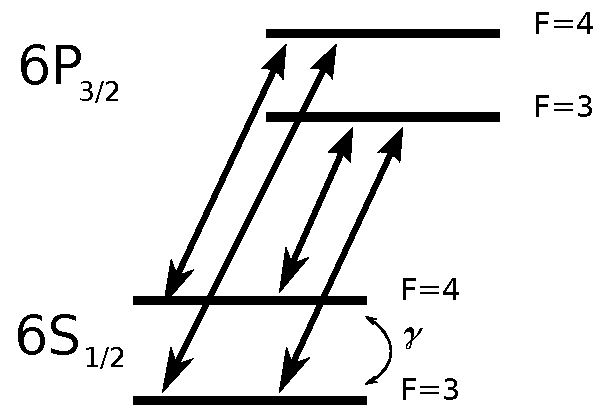
\includegraphics[width=.75\textwidth]{figures/simlevels}}
        \end{center}
      \end{figure}
    \end{column}
  \end{columns}

  \begin{itemize}
  \item Build-up time of the order of 1 ms
  \item No need for frequency offset locking
    \begin{itemize}
    \item slow centre frequency drift does not affect CPT signal
    \item offset dither not allowed
    \end{itemize}
  \item Reduced light shift and light broadening compared to CW, with small intensity dependence.
  \end{itemize}
  \begin{columns}
    \begin{column}{0.49\textwidth}
      \begin{figure}
        \begin{center}
          \setlength\fboxsep{0pt}
          \setlength\fboxrule{0.5pt}
          \fbox{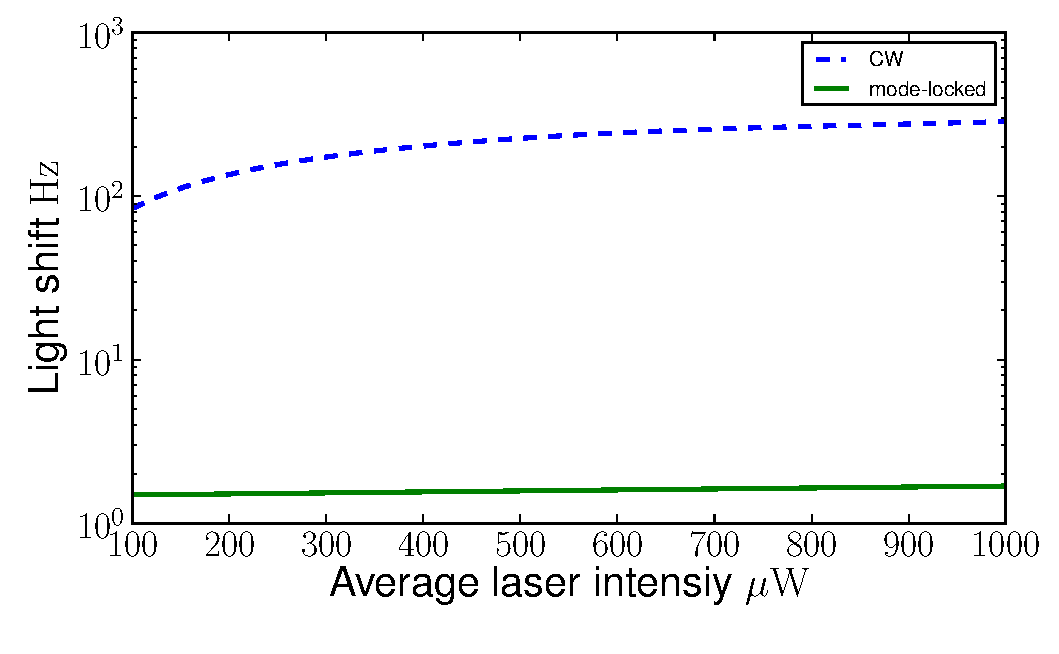
\includegraphics[width=.85\textwidth]{figures/lightshift}}
        \end{center}
      \end{figure}
    \end{column}
    \begin{column}{0.49\textwidth}
      \begin{figure}
        \begin{center}
          \setlength\fboxsep{0pt}
          \setlength\fboxrule{0.5pt}
          \fbox{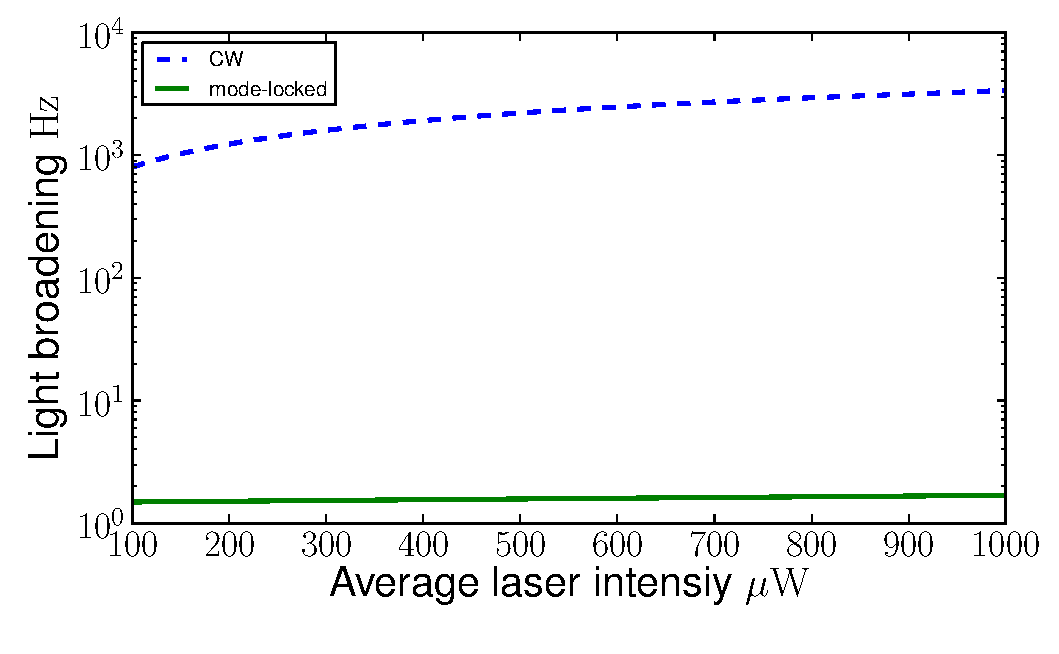
\includegraphics[width=.85\textwidth]{figures/lightbroad}}
        \end{center}
      \end{figure}
    \end{column}
  \end{columns}
  % %% Figures
  % \begin{figure}
  %   \includegraphics[width=0.5\textwidth]{}
  % \end{figure}
\end{block}


          }
        \end{minipage}
      \end{beamercolorbox}
    \end{column}
    % Right column
    \begin{column}{.49\textwidth}
      \begin{beamercolorbox}[center,wd=\textwidth]{postercolumn}
        \begin{minipage}[T]{.95\textwidth}
          % Parbox : to pull everything up to the top of the page, there might be better way than this
          \parbox[t][\columnheight]{\textwidth}{

            % Background
            \begin{block}{Background}
  \begin{figure}
    \begin{center}
      \includegraphics[width=.3\textwidth]{figures/energylevels}
      \caption{Energy levels}
    \end{center}
  \end{figure}
\end{block}

            \vfill

            % Experimental results
            \begin{block}{Experimental results}
  Put pretty pictures here
\end{block}

            \vfill

            % Future work, etc...
            \begin{block}{Outlook - the optical vernier}
  Our group developed compact frequency standards for two differen 2-photon Cs transitions (8S at 822 nm and 6D at 884 nm).
  \begin{columns}
    \begin{column}{0.60\textwidth}
     \begin{itemize}
     \item Extended cavity diode laser with intracavity cesium cell
     \item Focused beam for $\approx$ 1000 SNR for 822 nm
     \item Total length of 17 cm
     \end{itemize}
    \end{column}
    \begin{column}{0.39\textwidth}
      \begin{figure}
        \begin{center}
          \includegraphics[width=0.9\textwidth]{figures/compactreference}
        \end{center}
      \end{figure}
    \end{column}
  \end{columns}
  \begin{columns}
    \begin{column}{0.60\textwidth}
     \begin{itemize}
     \item   Combine this with a frequency comb to get an optical vernier.
       \begin{itemize}
       \item 822 nm reference locks the repetition rate
       \item 884 nm reference lock the absolute frequency
       \item CPT transition provides monitoring of the repetition rate, connecting the microwave and optical regime
       \end{itemize}
     \end{itemize}
    \end{column}
    \begin{column}{0.39\textwidth}
      \begin{figure}
        \begin{center}
          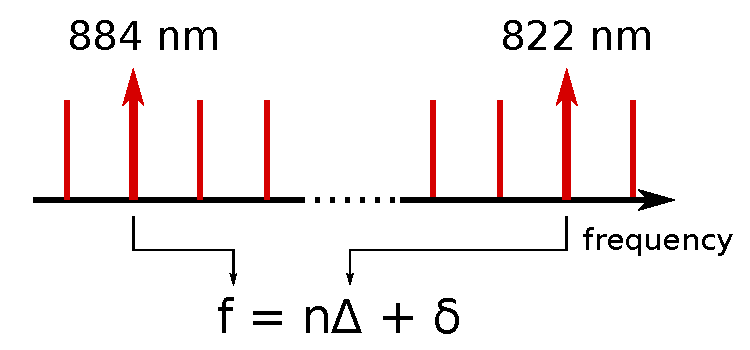
\includegraphics[width=1.0\textwidth]{figures/vernier}
        \end{center}
      \end{figure}
    \end{column}
  \end{columns}
  This scheme removes the need of a highly stable synthetizer, which is an obstacle to a compact and robust design.
\end{block}

          }
        \end{minipage}
      \end{beamercolorbox}
    \end{column}
  \end{columns}
%  \vskip1ex
\end{frame}
\end{document}


%%%%%%%%%%%%%%%%%%%%%%%%%%%%%%%%%%%%%%%%%%%%%%%%%%%%%%%%%%%%%%%%%%%%%%%%%%%%%%%%%%%%%%%%%%%%%%%%%%%%
%%% Local Variables: 
%%% mode: latex
%%% TeX-PDF-mode: t
%%% End:
